\documentclass[11pt, a4paper, oneside,UTF8]{ctexart}
\usepackage{amsmath,array, amsthm, amssymb, appendix, bm, graphicx, mathrsfs,subcaption,booktabs,tabularx,listings,xcolor,titling,fancyhdr,fontspec,lipsum,titlesec,setspace}
\usepackage[hidelinks]{hyperref}
\usepackage[a4paper]{geometry}
\usepackage{enumitem,lastpage}

% 设置页边距
\geometry{left=20mm,right=20mm,top=20mm,bottom=20mm}

% 设置页眉
\pagestyle{fancy}
\fancyhf{} % 清除当前设置的页眉和页脚
\cfoot{Page \thepage\ of \pageref{LastPage}} % 在页脚中间显示页码
\renewcommand{\headrulewidth}{0mm} % 设置页眉的分隔线粗细
\renewcommand{\footrulewidth}{0.1mm} % 设置页脚的分隔线粗细

% 设置 Fira Mono 字体
\setmonofont{Fira Mono}[Scale=0.9]

\title{\textbf{LLVM Pass Practice Report}}
\setlength{\droptitle}{-2cm}
\author{钟泓逸522031910522}
\date{}%
\linespread{1.5}
\newtheorem{theorem}{定理}[section]
\newtheorem{definition}[theorem]{定义}
\newtheorem{lemma}[theorem]{引理}
\newtheorem{corollary}[theorem]{推论}
\newtheorem{example}[theorem]{例}
\newtheorem{proposition}[theorem]{命题}
\renewcommand{\abstractname}{\Large\textbf{摘要}}
\pagestyle{plain}%

% 自定义标题格式
\titleformat{\section}[hang]{\normalfont\Large\bfseries}{\thesection}{1em}{}
\titleformat{\subsection}[hang]{\normalfont\large\bfseries}{\thesubsection}{1em}{}
\titleformat{\subsubsection}[hang]{\normalfont\normalsize\bfseries}{\thesubsubsection}{1em}{}

\definecolor{lightgray}{HTML}{EEEEEE}
\definecolor{darkgreen}{HTML}{4CAF50}
\lstset{
    language=C, % 设置语言为C
    backgroundcolor=\color{lightgray}, % 设置背景颜色
    basicstyle=\ttfamily\fontsize{10}{10}\selectfont, % 设置基本字体大小
    breaklines=true, % 自动断行
    showstringspaces=false, % 不显示字符串中的空格
    commentstyle=\color{darkgreen}, % 设置注释的颜色
    keywordstyle=\color{blue} % 设置关键字的颜色
}

\begin{document}
\setcounter{page}{1}

\maketitle
\vspace{-\baselineskip}
\thispagestyle{fancy}

\section{实验说明}
实验代码文件为\texttt{legacyArgCnt.cpp},\texttt{newArgCnt.cpp},以及相应的\texttt{CmakeLists.txt},放在llvm/lib/Transform/ArgCnt/文件夹下。

实验测试代码为\texttt{testcase1.c},以及相应文件\texttt{testcase1.ll},放在test文件夹下。

\section{基于legacy实现}

\subsection{引入所需库文件}

\begin{figure}[h]
    \centering
    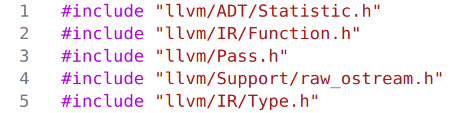
\includegraphics[width=0.5\textwidth]{./figure/legacy_1.png}
    \caption{include\_path}
    \label{figure:1.1}
\end{figure}

\begin{itemize}
    \setlength{\itemsep}{-1.0em}
    \item \texttt{llvm/ADT/Statistic.h}:用于统计信息的库
    \item \texttt{llvm/IR/Function.h}:Function抽象类,提供函数接口
    \item \texttt{llvm/Pass.h}:定义了pass的基本接口和方法
    \item \texttt{llvm/Support/raw\_ostream.h}:提供标准输入、标准输出接口
    \item \texttt{llvm/IR/Type.h}:提供Type类型
\end{itemize}

\subsection{FunctionPass实现}

具体结构实现如下图。

\begin{figure}[h]
    \centering
    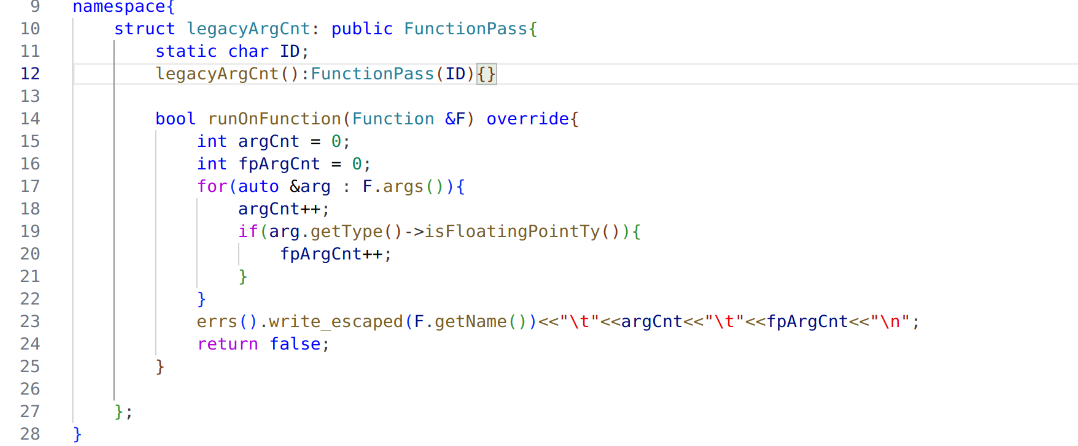
\includegraphics[width=0.5\textwidth]{./figure/legacy_2.png}
    \caption{legacyArgCnt结构}
    \label{figure:1.2}
\end{figure}

\textbf{总结构体概述:}
\begin{itemize}[before=\setstretch{0.9}]
    \setlength{\itemsep}{0em}
    \item \texttt{struct legacyArgCnt: public FunctionPass}:定义结构体\texttt{legacyArgCnt},继承自\texttt{FunctionPass},表示该pass作用于函数上,且函数之间相互独立。
    \item \texttt{static\ char ID}:定义了pass的唯一标识符ID
    \item \texttt{legacyArgCnt():FunctionPass(ID){}}:重载构造函数,用于构造legacyArgCnt结构体
    \item \texttt{bool runOnFunction(Function \&F) override}:定义FunctionPass实现的虚方法。
\end{itemize}

\textbf{runOnFunction概述:}
\begin{itemize}[before=\setstretch{0.9}]
    \setlength{\itemsep}{0em}
    \item 定义int变量\texttt{argCnt}、\texttt{fpArgCnt},用于参数和float\_pointing参数的计数
    \item \texttt{for(auto \&arg : F.args())}循环:用Function类的\texttt{arg()}函数获取参数列表,并进行遍历操作,每获取一个参数,\texttt{argCnt}计数增加,然后使用\texttt{getType()}函数获取当前arg的类型,并使用{isFloatingPointTy()}函数进行类型判断,若为FloatingPoint,则\texttt{fpArgCnt}计数增加。
    \item \texttt{errs().write\_escaped(F.getName())<<"\textbackslash t"<<argCnt<<"\textbackslash t"<<fpArgCnt<<"\textbackslash n";}:打印函数对应的名称和参数数量。
    \item \texttt{return false}:表示没有修改函数内容
\end{itemize}

\subsection{pass注册}

代码实现如下:

\begin{figure}[h]
    \centering
    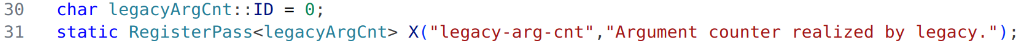
\includegraphics[width=0.5\textwidth]{./figure/legacy_3.png}
    \caption{RegisterPass}
    \label{figure:1.3}
\end{figure}

\begin{itemize}[before=\setstretch{0.9}]
    \setlength{\itemsep}{0em}
    \item \texttt{char legacyArgCnt::ID = 0}:定义pass的标识符ID,用于在pass管理系统中注册和识别该pass
    \item \texttt{static RegisterPass<legacyArgCnt> X("legacy-arg-cnt","Argument counter realized by \\legacy.")}:使用RegisterPass类来注册pass,并指定注册类型为legacyArgCnt,并定义命令行选项名称为legacy-arg-cnt,"Argument counter realized by legacy."定义了运行opt使用help选项时打印的帮助信息。
\end{itemize}

\section{基于new\_pass\_manager的实现}

\subsection{引入头文件}

\begin{figure}[h]
    \centering
    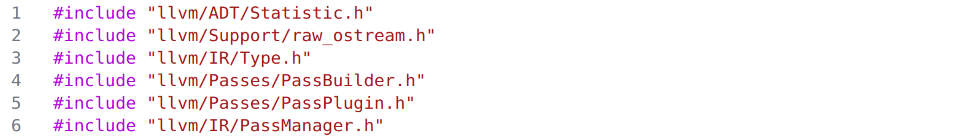
\includegraphics[width=0.5\textwidth]{./figure/new_1.png}
    \caption{include\_path}
    \label{figure:2.1}
\end{figure}

\begin{itemize}[before=\setstretch{0.9}]
    \setlength{\itemsep}{0em}
    \item \texttt{llvm/Passes/PassBuilder.h}: 构建pass管理器,用于注册和安排pass
    \item \texttt{llvm/Passes/PassPlugin.h}:定义和注册新的 LLVM Pass 插件,使得自定义pass能动态加载到llvm中
    \item \texttt{llvm/IR/PassManager.h}:提供新式pass管理器
\end{itemize}

\subsection{Pass实现}

具体结构定义如下。

\begin{figure}[h]
    \centering
    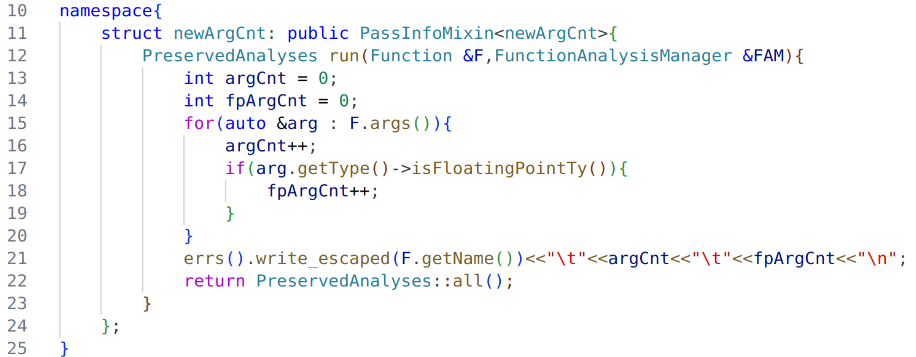
\includegraphics[width=0.5\textwidth]{./figure/new_2.png}
    \caption{newArgCnt实现}
    \label{figure:2.2}
\end{figure}

\textbf{结构概述}
\begin{itemize}[before=\setstretch{0.9}]
    \setlength{\itemsep}{0em}
    \item \texttt{struct newArgCnt: public PassInfoMixin<newArgCnt>}:定义结构体\texttt{newArgCnt},继承自新式pass管理器类\texttt{PassInfoMixin}
    \item \texttt{PreservedAnalyses run(Function \&F, FunctionAnalysisManager \&FAM)}:定义实现方法,该方法为每个函数上执行pass的实现逻辑。FAM是函数分析管理,用于获取和管理函数的分析结果。
    \item \texttt{}
\end{itemize}

\textbf{run函数概述}
\begin{itemize}[before=\setstretch{0.9}]
    \setlength{\itemsep}{0em}
    \item 函数信息的统计和打印与legacy方法实现相同
    \item \texttt{PreservedAnalyses::all()}:表示这个 Pass 没有改变任何分析结果
\end{itemize}

\subsection{Pass的注册与加载}

\begin{figure}[h]
    \centering
    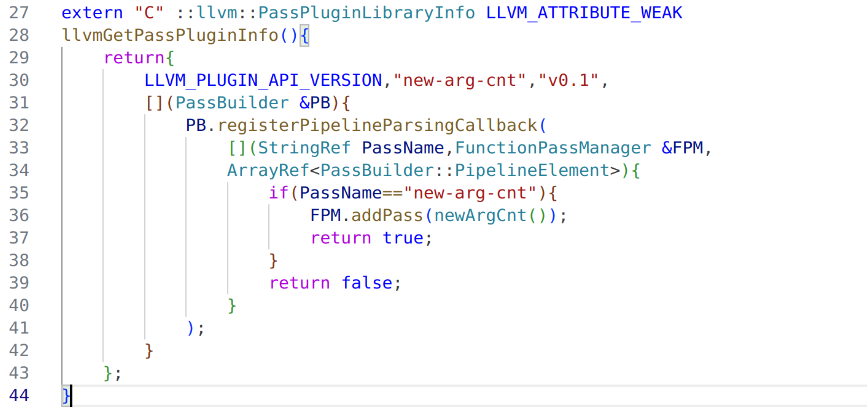
\includegraphics[width=0.5\textwidth]{./figure/new_3.png}
    \caption{pass插件的注册与加载}
    \label{figure:2.3}
\end{figure}

\begin{itemize}[before=\setstretch{0.9}]
    \setlength{\itemsep}{0em}
    \item \texttt{::llvm::PassPluginLibraryInfo LLVM\_ATTRIBUTE\_WEAK}:定义了PassPluginLibraryInfo,用于描述pass插件的版本和注册信息,LLVM\_ATTRIBUTE\_WEAK声明了弱链接,使得插件可以在链接阶段动态加载。
    \item \texttt{llvmGetPassPluginInfo()}:声明该结构体的初始化函数
    \item \texttt{LLVM\_PLUGIN\_API\_VERSION,"new-arg-cnt","v0.1"}:定义了插件的名称和版本
    \item \texttt{[](PassBuilder \&PB)}:定义pass构建器,用于构建和注册pass
    \item \texttt{registerPipelineParsingCallback}:注册回调函数
    \item \texttt{[](StringRef PassName, FunctionPassManager \&FPM, ArrayRef<PassBuilder::PipelineElement>) { ... }}:定义回调函数体,当解析到pass名称为new-arg-cnt时,向pass管理器中增加一个newArgCnt的pass实例,并且返回true表示成功注册了pass
    
\end{itemize}

\section{测试案例}

测试案例中定义两个函数:test1aaa,test2bbb。具体代码如下:

其中test1aaa共有3个参数,其中1个fp类型参数;test2aaa共有3个参数,其中2个fp类型参数。

\begin{figure}[h]
    \centering
    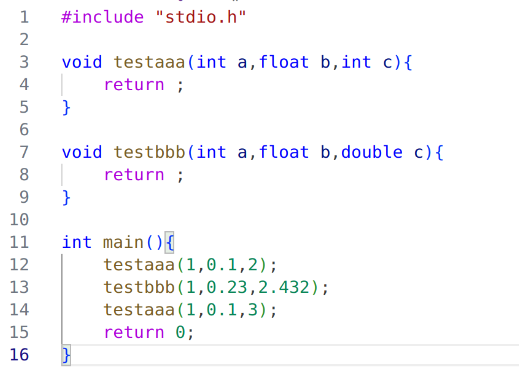
\includegraphics[width=0.5\textwidth]{./figure/test_1.png}
    \caption{testcase1.c}
    \label{figure:3.1}
\end{figure}

执行指令\texttt{\$ ../build/install/bin/clang -O0 -emit-llvm -S testcase1.c -o testcase1.ll},将c文件转换成ll文件,看到转换后的文本如下。
\begin{figure}[h]
    \centering
    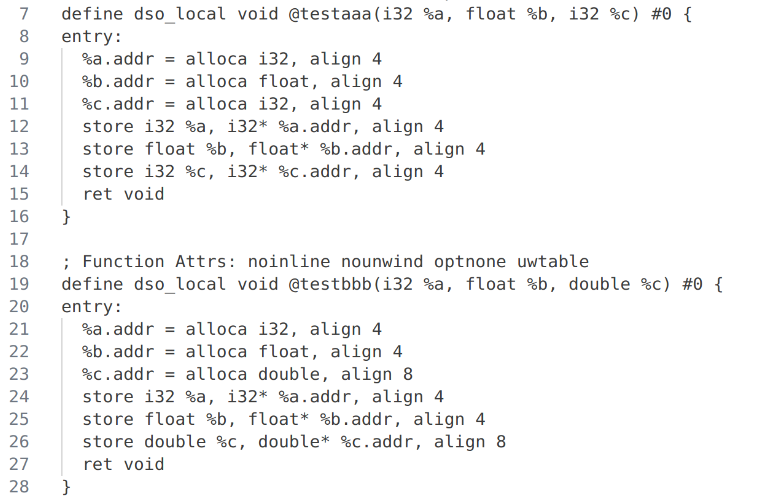
\includegraphics[width=0.7\textwidth]{./figure/test_2.png}
    \caption{testcase1.ll}
    \label{figure:3.2}
\end{figure}

\section{实验结果验证}

首先,添加CmakeLists.txt,编译legacyArgCnt.cpp和newArgCnt.cpp成libFuncArgCnt模块。
\begin{figure}[h]
    \centering
    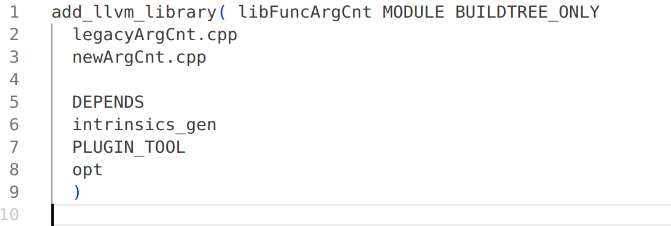
\includegraphics[width=0.5\textwidth]{./figure/cmake_1.png}
    \caption{CmakeLists.txt}
    \label{figure:4.1}
\end{figure}

然后在Transform文件夹修改CmakeLists.txt,添加\texttt{add\_subdirectory(ArgCnt)}。编译文件后得到动态库。

在test文件夹下执行指令,分别使用new-arg-cnt和legacy-arg-cnt,获得优化输出信息:

\begin{figure}[h]
    \centering
    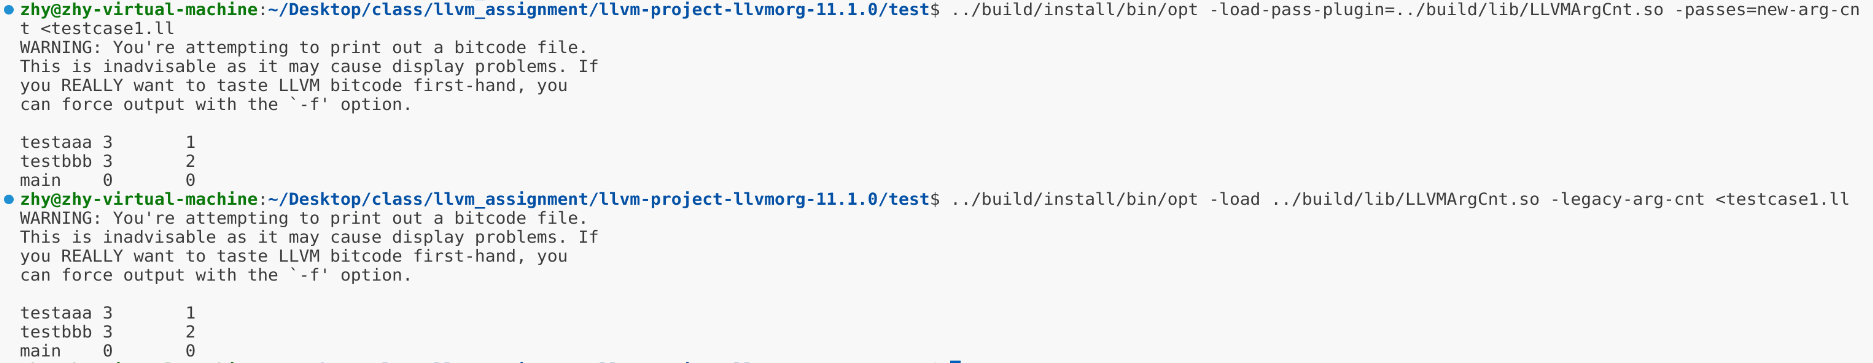
\includegraphics[width=1\textwidth]{./figure/result.png}
    \caption{实验结果}
    \label{figure:5.1}
\end{figure}
则pass处理时正确输出了函数名以及对应参数数量。

\end{document}